In this section we describe the dataset we used for our experiments. 
The dataset consists of both electricity consumption and weather data, collected from various sources. 
The electricity consumption data was obtained from the Israeli electricity system operator Noga~(\cite{noga}), 
while the weather data was sourced from a nearby meteorological station~(\cite{ims}).
Electricity consumption data includes hourly readings of power usage.
Crucially, it also includes the \emph{real day-ahead forecasts} published by Noga as part of the
market clearing process.  These are the actual forecasts used by the system operator in the
day-ahead market, not post-hoc reconstructions.  Their inclusion in our dataset
provides two important opportunities: (i)~we can directly compare the performance
of our learned models against the operational forecasts actually used in the market,
serving as a strong real-world baseline; and (ii)~we can analyze the
distribution of real-world prediction errors produced by an experienced operator,
which motivates and contextualizes the cost asymmetries studied in this paper.
The weather data includes temperature, humidity, and wind speed measurements taken every three hours in the three major cities of Israel: Tel Aviv, Jerusalem, and Haifa.
% Table~\ref{tab:electricity-fields} summarizes the fields present in the electricity consumption data,
% and Table~\ref{tab:weather-fields} summarizes the fields present in the weather data. 
% The dataset covers the period from March 2023 to February 2026, 
% providing a comprehensive view of electricity consumption patterns 
% and their relationship with weather conditions over the course of almost three years.

% \begin{table}[ht]
%     \centering
%     \begin{tabular}{ll}
%         \hline
%         \textbf{Field} & \textbf{Description} \\
%         \hline
%         \texttt{date} & Calendar date (DD-MM-YYYY). \\
%         \texttt{total\_demand} & Total daily electricity demand (MWh). \\
%         \texttt{total\_day\_ahead\_forecast} & Operator's day-ahead forecast (MWh). \\
%         \hline
%     \end{tabular}
%     \caption{Electricity consumption data fields (daily aggregated from hourly source data).}
%     \label{tab:electricity-fields}
% \end{table}

% \begin{table}[ht]
%     \centering
%     \begin{tabular}{ll}
%         \hline
%         \textbf{Field} & \textbf{Description} \\
%         \hline
%         \texttt{temperature\_Haifa} & Daily mean temperature, Haifa ($^\circ$C). \\
%         \texttt{temperature\_Jerusalem} & Daily mean temperature, Jerusalem ($^\circ$C). \\
%         \texttt{temperature\_Tel\_Aviv} & Daily mean temperature, Tel~Aviv ($^\circ$C). \\
%         \hline
%     \end{tabular}
%     \caption{Weather data fields (daily means aggregated from tri-hourly station observations).}
%     \label{tab:weather-fields}
% \end{table}

\subsection{Data Analysis}
To better understand the dataset, we performed an exploratory data analysis (EDA) to identify patterns and relationships between the electricity consumption and weather data.
Figure~\ref{fig:daily-demand} shows the daily electricity consumption over the course of the dataset alongside the daily average temperature in Tel Aviv.

\begin{figure}[ht]
    \centering
    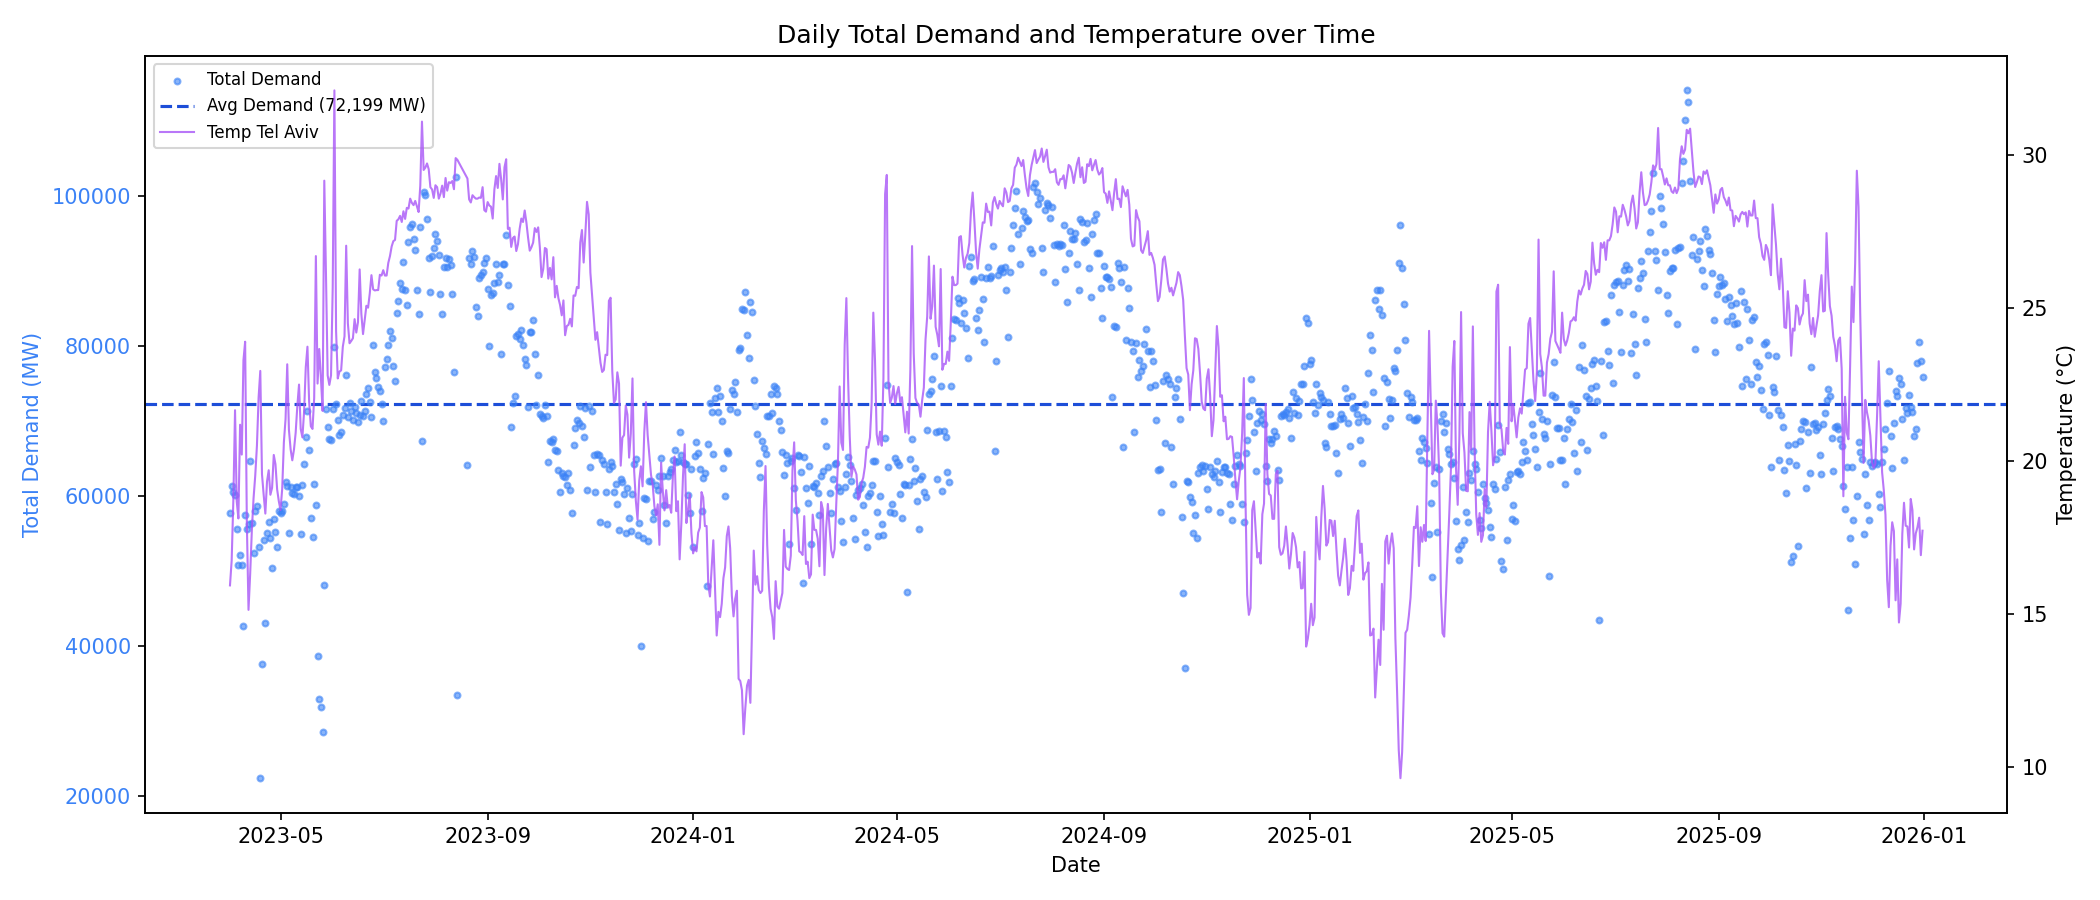
\includegraphics[width=\textwidth]{plot/daily_demand_by_time.png}
    \caption{Daily electricity consumption (MWh) over the dataset period
    (March~2023--February~2026).  Clear seasonal patterns are visible, with
    a summer peak (July--August) driven by air-conditioning loads and a secondary
    winter peak (January--February) driven by heating.}
    \label{fig:daily-demand}
\end{figure}

Figure~\ref{fig:daily-demand-vs-temp} shows the relationship between daily electricity consumption and the daily average temperature in Tel Aviv.

\begin{figure}[ht]
    \centering
    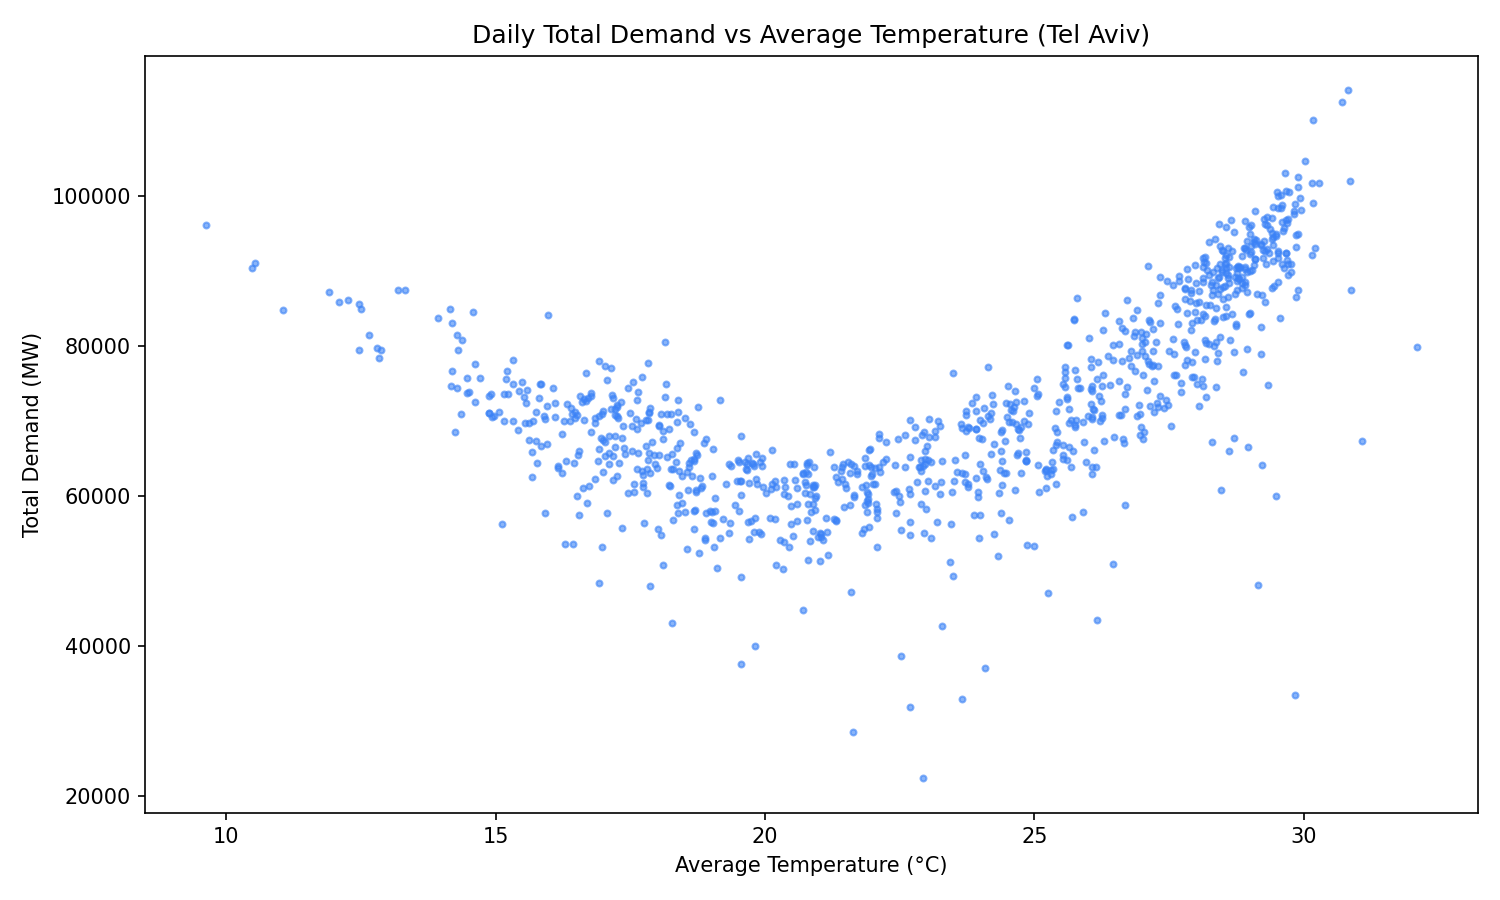
\includegraphics[width=\textwidth]{plot/daily_demand_vs_avg_temp_Tel_Aviv.png}
    \caption{Daily electricity consumption vs.\ daily mean temperature in
    Tel~Aviv.  The characteristic U-shaped relationship is visible, with
    high demand at both high temperatures (cooling loads) and low temperatures
    (heating loads).  The balance-point temperature is approximately
    20\,$^\circ$C.}
    \label{fig:daily-demand-vs-temp}
\end{figure}

% Figure~\ref{fig:daily-demand-vs-forecast-time} depicts the relationship between daily electricity consumption and the operator's day-ahead forecast over time.

% \begin{figure}[ht]
%     \centering
%     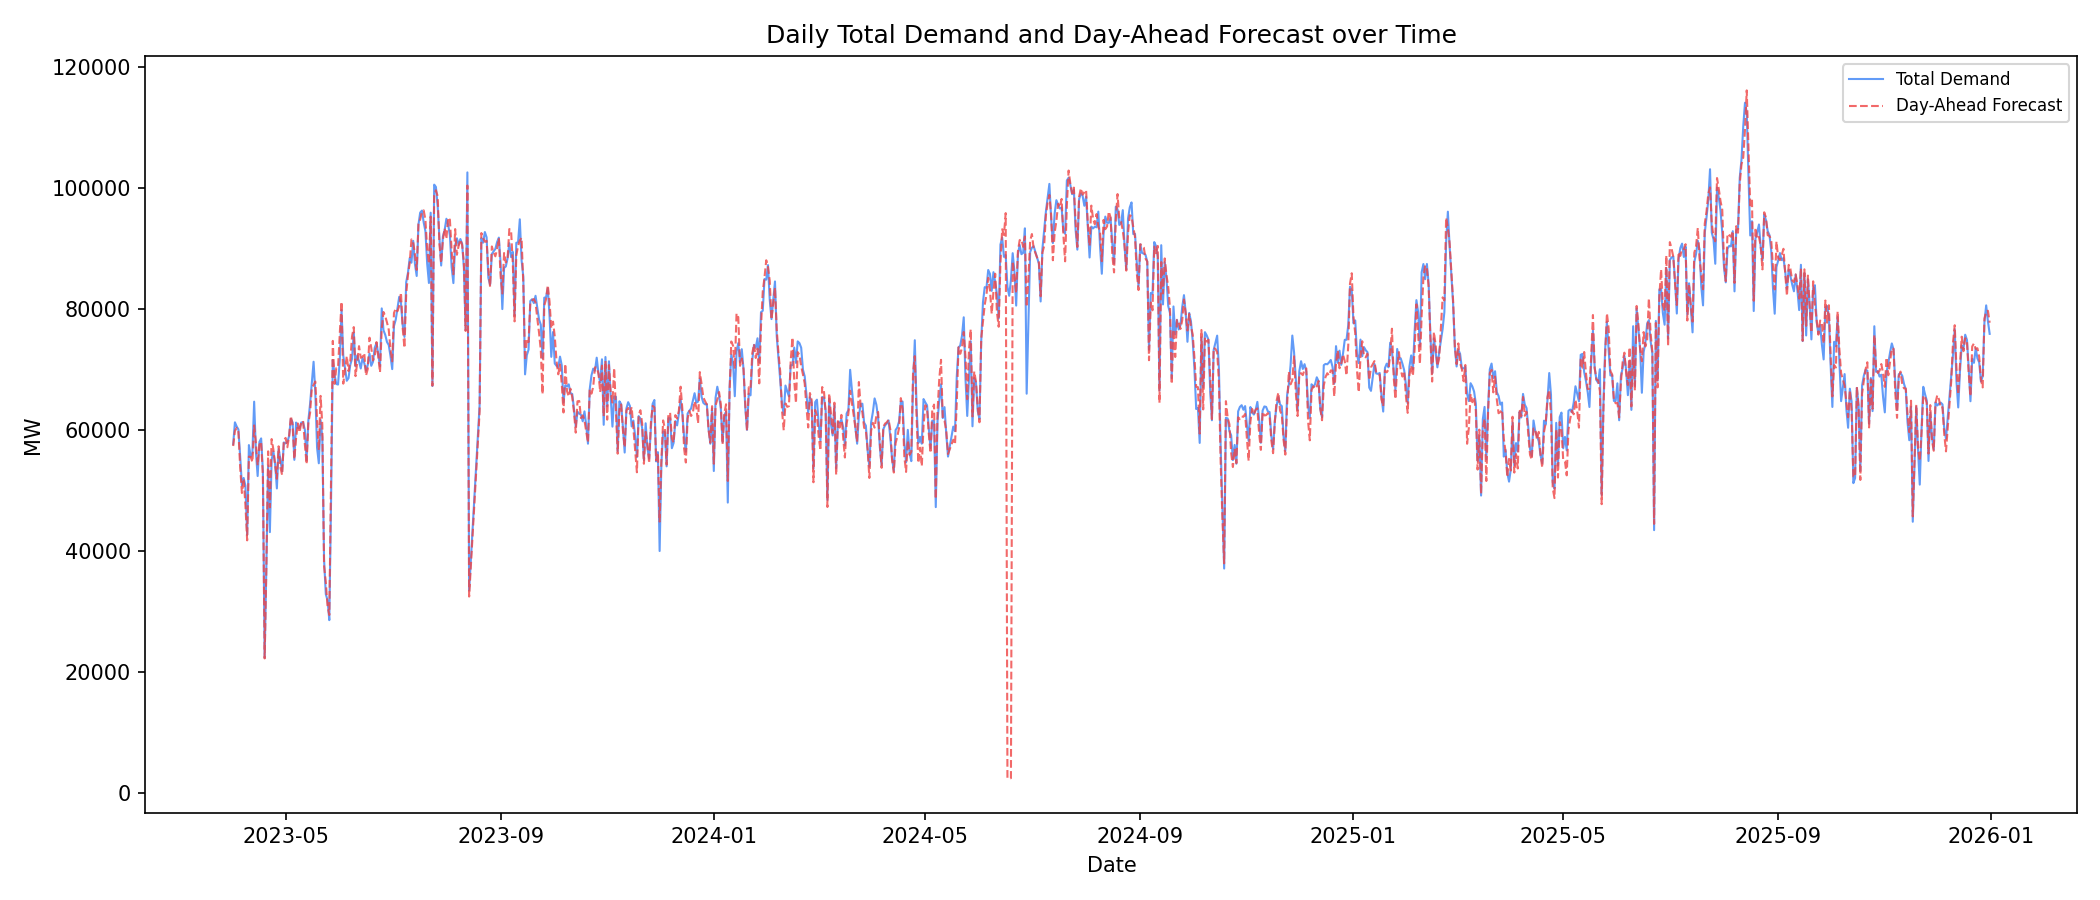
\includegraphics[width=\textwidth]{plot/daily_demand_vs_forecast_time.png}
%     \caption{Daily electricity consumption (solid blue) vs.\ operator day-ahead
%     forecast (dashed orange) over time.  The forecast tracks actual demand
%     closely, with visible errors during demand spikes.}
%     \label{fig:daily-demand-vs-forecast-time}
% \end{figure}

Figure~\ref{fig:demand-vs-forecast-kde} shows the KDE histogram of the forecast error, i.e., the difference between the actual demand and the day-ahead forecast.

\begin{figure}[ht]
    \centering
    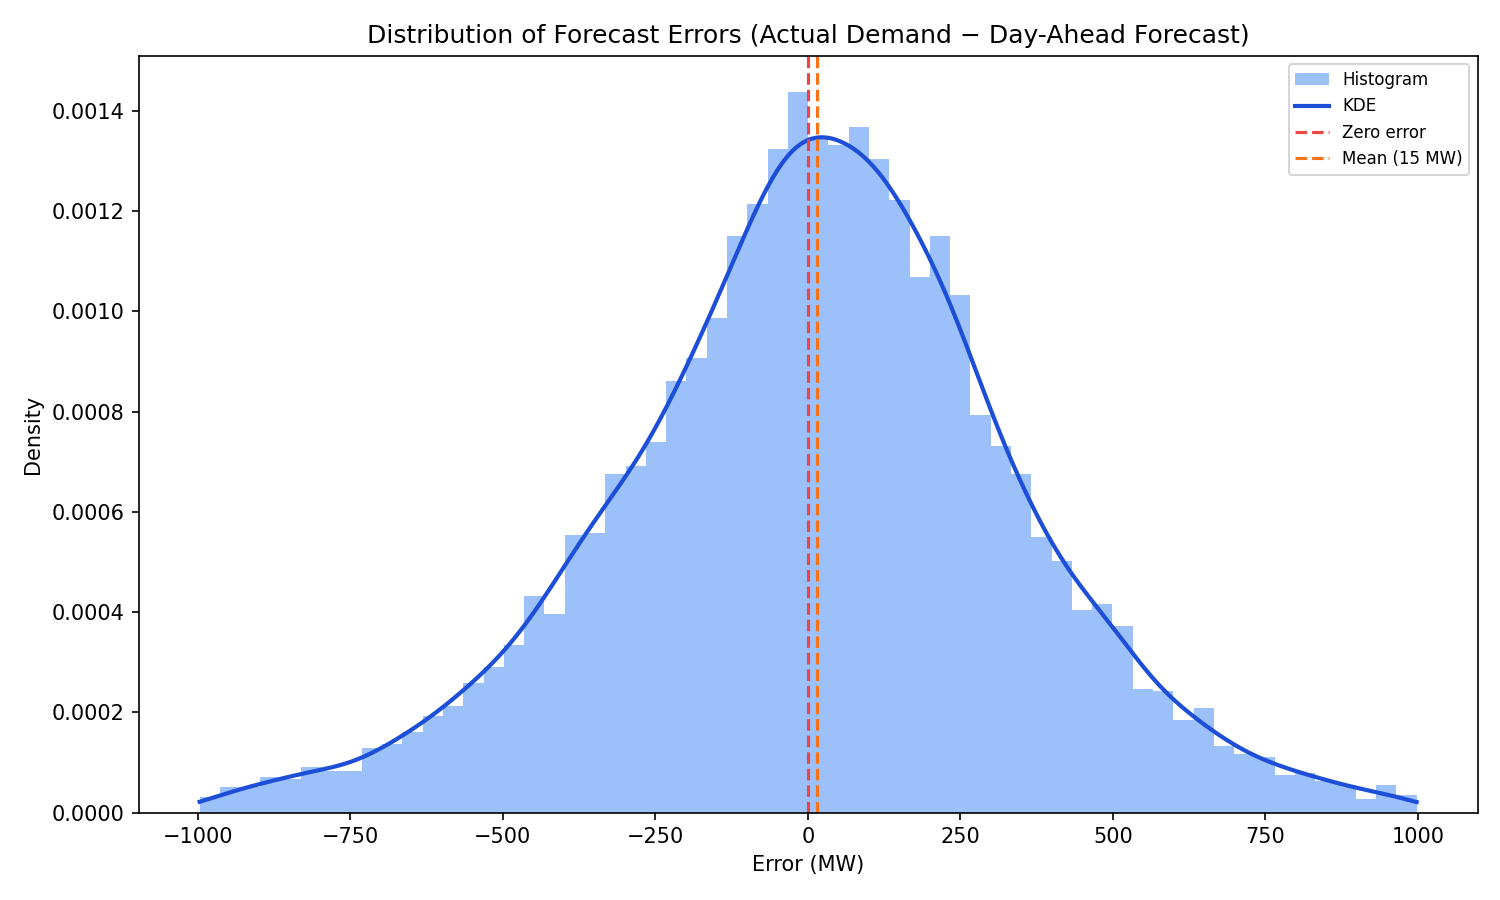
\includegraphics[width=\textwidth]{plot/demand_vs_forecast_kde_histogram.png}
    \caption{KDE histogram of the forecast error (actual demand minus
    day-ahead forecast).  The distribution is approximately zero-mean with
    slightly heavier right tails, suggesting that large under-forecasts are
    marginally more frequent than large over-forecasts.}
    \label{fig:demand-vs-forecast-kde}
\end{figure}

% \subsection{Dataset Statistics}

Table~\ref{tab:dataset-stats} reports summary statistics for the key variables in
the daily dataset.  The data span 1{,}096~days from 1~March~2023 to
28~February~2026.

\begin{table}[ht]
    \centering
    \begin{tabular}{lrrrrr}
        \toprule
        \textbf{Variable} & \textbf{Mean} & \textbf{Std} &
        \textbf{Min} & \textbf{Median} & \textbf{Max} \\
        \midrule
        Total demand (MWh) & 73\,421 & 14\,852 & 19\,742 & 70\,435 & 114\,103 \\
        Day-ahead forecast (MWh) & 73\,109 & 14\,680 & 2\,400$^{*}$ & 70\,200 & 116\,148 \\
        Forecast error (MWh) & $+312$ & 3\,241 & $-12\,300$ & $+284$ & $+11\,543$ \\
        Temp.\ Tel~Aviv ($^\circ$C)    & 22.1 & 4.8 &  9.6 & 22.5 & 30.3 \\
        Temp.\ Jerusalem ($^\circ$C)   & 18.9 & 6.4 &  2.3 & 19.8 & 36.5 \\
        Temp.\ Haifa ($^\circ$C)       & 20.3 & 5.1 &  4.4 & 20.8 & 31.3 \\
        \bottomrule
    \end{tabular}
    \caption{Summary statistics for daily variables ($N = 1{,}096$ days,
    March~2023--February~2026).
    $^{*}$Three anomalous forecast values excluded from statistics; see text.}
    \label{tab:dataset-stats}
\end{table}

\subsection{Seasonal and Weekly Patterns}

Israel's electricity demand exhibits well-defined seasonal and intra-week
patterns driven by climate, culture, and the structure of the working week.

\textbf{Seasonal patterns.}  The Mediterranean climate produces a pronounced
summer peak (July--August) driven by air-conditioning loads, and a secondary
winter peak (January--February) driven by heating.  Demand troughs in the mild
spring and autumn shoulder seasons.  This ``double-peak'' profile is visible in
Figure~\ref{fig:daily-demand}.

\textbf{Weekly patterns.}  Unlike most European countries, the Israeli working
week runs Sunday through Thursday; Friday is a short workday and Saturday
(Shabbat) is the day of rest.  Consequently the lowest-demand day of the week is
Saturday, followed by Friday, rather than Sunday.

\begin{figure}[ht]
    \centering
    \includegraphics[width=\textwidth]{plot/demand_by_day_of_week.png}
    \caption{Mean daily electricity demand by day of the week (box plots over
    the full dataset period).  Saturday (Shabbat) is the lowest-demand day,
    followed by Friday; Sunday is the first working day and shows a marked
    demand increase.  This shift relative to the European weekend structure
    means that standard day-of-week features must be recoded to reflect the
    Israeli calendar, and motivates the inclusion of a dedicated
    weekend/holiday indicator in our feature representation.}
    \label{fig:demand-by-dow}
\end{figure}

\textbf{Temperature sensitivity.}  Figure~\ref{fig:daily-demand-vs-temp} shows
the characteristic U-shaped demand--temperature relationship, with high demand
at both high temperatures (cooling) and low temperatures (heating).  The
balance point (minimum demand) occurs at approximately 18\,$^\circ$C in Tel~Aviv.
The very high air-conditioning penetration ($>\!95$\% of households) makes
summer peak demand extremely sensitive to temperature, complicating forecasting
during heat waves.

\subsection{Forecast Error Distribution}

As shown in Figure~\ref{fig:demand-vs-forecast-kde}, the Noga day-ahead forecast
errors (actual minus forecast) are strikingly close to zero-mean and nearly
symmetric: the mean error is only $+312$~MWh against a standard deviation of
$3{,}241$~MWh, and the KDE is approximately bell-shaped with modest skewness.
In other words, the operational forecast is essentially unbiased, under-predicting
and over-predicting with roughly equal frequency and magnitude.

From a pure accuracy standpoint this is a desirable property.  From a
cost-sensitive standpoint, however, it is a warning sign.  As established in
Section~\ref{sec:modeling}, when the costs of under-prediction substantially
exceed those of over-prediction the cost-minimising forecast is \emph{not} the
conditional mean but a higher quantile --- a deliberate upward bias proportional
to the cost asymmetry.  An approximately symmetric, zero-mean forecast therefore
fails to account for the asymmetric cost structure of the market, and will
systematically incur higher expected operational cost than a cost-aware
alternative.  This observation is central to the motivation of our approach and
is quantified empirically in Section~\ref{sec:evaluation}.

\subsection{Comparison with the Noga Operational Forecast}

A distinctive feature of our dataset is the availability of the \emph{real}
day-ahead forecasts produced by Noga and used in the actual electricity market.
This allows us to evaluate our learned models not merely against simple
statistical baselines but against the operational forecast of an experienced
system operator with access to proprietary data and domain expertise.

The Noga forecast achieves $R^2\approx 0.98$ against actual demand, confirming it is a strong accuracy baseline.  
Its error distribution is, as discussed in Section~\ref{sec:forecast-error-dist}, nearly zero-mean and approximately symmetric.  
While this is impressive from an accuracy standpoint, it also
reveals a limitation: the Noga forecast behaves as a conditional-mean estimator, making no explicit adjustment for cost asymmetry.  
A symmetric, unbiased forecast minimises mean squared error but, as we show empirically in
Section~\ref{sec:evaluation}, it does \emph{not} minimize expected operational
cost when under-prediction is substantially more costly than over-prediction.
Its high $R^2$ is therefore a misleading indicator of operational performance
under asymmetric costs --- a point that motivates the cost-sensitive approach
developed in this paper.

